\mychapter{implementation}{Implementation/realization - cloudml-engine}

In the previous chapter the design of CloudML was introduced.
In this chapter the implementation of this design will be presented and described.
First section is a technical overview of some of the general solutions within 
the implementation.
The rest of the chapter is split into different sections, one for each important part of the implementation.
Topics are about
\begin{ii}
  \iitem submodules and their tasks,
  \iitem the depdency system,
  \iitem communication with cloud providers,
  \iitem \myac{M@RT} through actor model and
  \iitem data serialization.
\end{ii}

\mysection{technologies}{Technology overview}

CloudML is implemented as a \emph{proof-of-concept} framework~\cite{cloudml-engine}
(from here known as \emph{cloudml-engine}). 
The implementation, \emph{cloudml-engine}, 
is based on \emph{state-of-the-art} technologies that appeal to the academic community.
Technologies chosen for \emph{cloudml-engine} are not of great importance to the concept of CloudML itself,
but it is still important to understand which technologies are chosen, what close alternatives exists
and why they are chosen.

\paragraph{Language and environment.} 

The importance of a \emph{programming language} and \emph{environment} were
described in \citesec{technological-assessments}.
These are core ideas to fulfill \citereq{foundation}, emphasizing the importance of a strong foundation.
Here is a list describing some of the languages and environments considered:
\begin{itemize}
  \item Java (\myac{JVM})
  \item JavaScript (Node.js)
  \item Scala (\myac{JVM})
  \item Python
  \item C\# (.NET)
\end{itemize}
Languages in this list are introduced because of their overall popularity.
Some were introduced despite this, such as \emph{Node.js}, 
which is brought in as an consideration because of the abilities to operate
with \myac{JSON}, cloud interaction and modernity.

Based on these considerations Scala is a good choice, it fulfills the core ideas and match
the requirement \citereq{foundation}:
\begin{description} 
  \item[Ease of use.]
    Scala is a \emph{state-of-the-art} language with many technological advantages,
    \eg supporting both functional and object-oriented programming.
    With both paradigms, imperative programmers such as Java developers as well as functional
    programmers such as Clojure developers would be familiar with the language design.
    
    Emphasizes on functional programming which is leveraged in the implementation.
    Built in system for actor model~\cite{actors:haller07}, which is utilized in the implementation.
    This also assists in relation to \citereq{m@rt}.

    \myac{JVM} is a popular platform, as the main platform for Java.
    Scala runs on the \myac{JVM}, and support all the libraries and work put into Java
    over the years can be utilized directly by Scala.
  \item[Community size.]
    This language is gaining popularity among both the academic and enterprise domain.
  \item[Closed/open source.] Scala is open source.
  \item[Modernity.]
    The reason not to use plain Java is because Scala is an appealing \emph{state-of-the-art} language.
    The language is under constant development and new features and enhancements keeps improving
    the language.
  \item[Matureness.]
    Compatible with Java and libraries written in Scala can be interacted with by Java as well.
    This means that even though Scala is chosen for the implementation of CloudML,
    it can still be used by other languages supported by the \myac{JVM},
    \eg Java, Groovy and Clojure.
\end{description}
Based on these benefits Scala is chosen, and \emph{cloudml-engine} is written in this language.


\mysection{dependencies}{Automatic build system}
\begin{figure}[tb]
  \subfigure[dependency-graph-without-test] {
    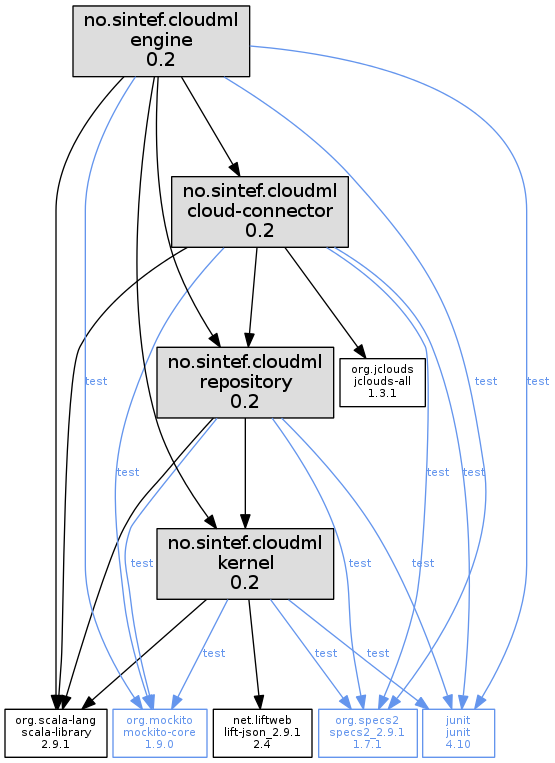
\includegraphics[width=8cm]{imgs/dependency-graph-2.png}
    \label{fig:dependency-graph-without-test}
  }
  \subfigure[dependency-graph-with-test] {
    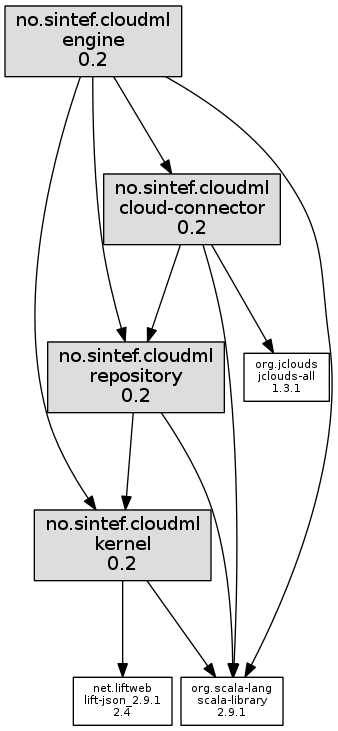
\includegraphics[width=5cm]{imgs/dependency-graph-1.png}
    \label{fig:dependency-graph-with-test}
  }
  \caption{Maven dependency graph (with and without test scope).}
  \label{fig:dependency-graph}
\end{figure}


%this is a \emph{Scala Object} used to initialize provisioning.
%A \emph{Scala Object} works as a \emph{singleton}, 

There are two main methods used to automatically build Scala programs, 
either using a Scala-specific tool called \myac{SBT} or a more general tool called Maven. 
For \emph{cloudml-engine} to have an academic appeal it is essential to choose the technology
with most closeness to Java, hence Maven is the best option.
It is also important to make the library available for developers using Java or other
languages supported by the \myac{JVM}.
This is best achieved by using Maven, as \myac{SBT} is directed at Scala.

In \citesec{modules} CloudML were split into four different modules, as seen in \citefig{cloudml-modules}.
Maven support modules, these are used to split \emph{cloudml-engine} into the appropriate 
modules.

A full Maven dependency graph is expressed in \citefig{dependency-graph}.
There are two graphs, both of \emph{cloudml-engine}.
The first graph~(\citefig{dependency-graph-without-test}) excludes the \emph{test-scope},
while~\citefig{dependency-graph-with-test} includes it.
The \emph{test-scope} is a Maven scope which marks the dependencies to only be included
when running a specific \emph{goal}, \eg test.
In this graph the internal and external dependencies in \emph{cloudml-engine} are expressed.
All external dependencies, 
\eg \texttt{org.jclouds.jclouds-all}~(\citefig{dependency-graph}),
contain even more dependencies to other libraries and internal modules.
These dependencies are all omitted in both graphs.

%The dependencies are defined in \emph{pom.xml}-files.
%Parts of a dependency reference in a Maven configuration can be seen in~\citefig{pom-example},
%although this is not dependency management in between \emph{cloudml-engine} modules but rather
%how to add \emph{cloudml-engine} as a dependency itself.

\section{Cloud connection}

The connection between CloudML and cloud providers is facilitated 
to a separate module, called \texttt{cloud-connector}.
In the implementation this module is the bridge between providers and \emph{cloudml-engine}.
It is built to support several libraries and interface these,
this is achieved by implementing a type of \emph{facade pattern}.
It does not contain any entities, and only executes logical code. 

The bridge between \emph{cloudml-engine} and cloud providers is an important aspect of the application, 
and as a requirement it is important to use an existing library to achieve this connection.
Some libraries have already been mentioned in the \emph{APIs} section~(\citesec{API}),
of these only \emph{jclouds} is based on Java-technologies and therefore suites \emph{cloudml-engine}.
This library gives CloudML support for 24 providers out of the box to minimize \emph{complexity},
as well as stability and robustness.
These advantages directly resolves resolves \citereq{software-reuse}.
Jclouds uses Maven for building as well, and is part of Maven central which makes 
it possible to add jclouds directly as a module dependency.
Jclouds contains a template system which is used through code directly, this is utilized 
to map CloudML templates to jclouds templates.

\section{Asynchronous provisioning}

Provisioning can consume up to minutes for each instance,
it is therefore essential to make use of asynchronous behavior.
The solution, \emph{coudml-engine}, combines two different approaches to achieve this,
actor model and observer pattern.

\paragraph{Actor model.}

The asynchronous solution in CloudML is based on actor model~\cite{actors:haller07},
resulting in concurrent communication with nodes under provisioning.
By adopting this behavior developers exploring the implementation can then choose
to ``listen'' for updating events from each node,
and do other jobs / idle while the nodes are provisioned.

The actor model in CloudML is based on built-in implementations in Scala, 
\texttt{scala.actor.Actor}.
This approach solves \citereq{foundation},
as the underlying technology provides the asynchronous solution.
The actor model could be implemented using external libraries instead,
\eg Akka,
in this case the approach would solve \citereq{software-reuse}.

\paragraph{Observer pattern.}

Beside the standard model provided by Scala \emph{cloudml-engine} uses
a callback-based pattern to inform users of the library when instance statues
are updated and properties are added.

\paragraph{Models@run.time.}

The terms are divided for a node before and under provisioning, the essential is to introduce 
\emph{M@RT} to achieve a logical separation.

\section{From text to objects}
\begin{table}
  \begin{tabular*}{\textwidth}{@{\extracolsep{\fill}}| l | l | l | l |}
      \hline
        \textbf{Requirement} & 
        \textbf{XML} & 
        \textbf{JSON} &
        \textbf{YAML} \\
      \hline
        Community & $2$ & $2$ & $1$ \\ \hline
        Technology support & $2$ & $2$ & $1$ \\ \hline
        Human-readable & $1$ & $2$ & $3$ \\ \hline
        Web-service friendly & $2$ & $2$ & $0$ \\ \hline
  \end{tabular*}
  \caption{Comparing lexical formats (\citesec{technological-assessments})
    with aspects from requirement \citereq{lexical-template}.
    Weighting from zero ($0$) to three ($3$) respectively least to most supported.}
  \label{table:requirements-lexical}
\end{table}



As described in \citechap{requirements} there exists numerous implementations of different lexical formats.
Three of these formats are chosen as the most important ones,
\begin{ii}
  \iitem XML,
  \iitem JSON and
  \iitem YAML.
\end{ii}
The most important points about these formats are described in \citesec{technological-assessments},
\ie
\begin{ii}
  \iitem community,
  \iitem technology support,
  \iitem human-readable and
  \iitem web-service friendly.
\end{ii}
The different points are expressed in \citetable{requirements-lexical}, 
compared against the three different formats.
In the table they are weighted from zero ($0$) to three ($3$),
where zero is least supported and three is most supported,
\ie how well the formats cover the aspects described in \citesec{technological-assessments}.

For the lexical representation of CloudML, \myac{JSON} is the best alternative.
This format is used because of the values seen in \citetable{requirements-lexical}.

Here is an extracted list of the most relevant points compared against the \myac{JSON} format:
\begin{description}
  \item[Community.] This format is growing in popularity as more adapt to using it for
    different purposes, \eg databases, web-service communications, configuration files or \myac{i18n}.
  \item[Technology support.]
    There exists parsing libraries for most languages,
    for each of the languages listed in \citesec{technologies}.
  \item[Human-readable.]
    The format itself does not have any duplications, and is therefore easier read by humans
    than \myac{XML}.
  \item[Web-service friendly.]
    Used for both communicating between browsers and web servers, 
    and interchange between nodes in a \myac{SOA} environment.
\end{description}
%\begin{description}
%  \item[XML.] A well-known format in both academic domain and industry.
%    It is used by and for many different applications and tools for tasks such as configuration,
%    rendering and data exchange.
%    It is human-readable to some extent, but it is difficult with larger data sets because
%    of factors such as \emph{duplication} (node names are duplicated for termination). 
%    The markup is often used in web services, for instance in SOAP, 
%    and it was the initial data exchange format for \myac{XHR} (AJAX).
%  \item[JSON.] T
%  \item[YAML.] Strong focus on human-readability, by removing characters that can seem
%    distracting for the human eye, \eg brackets and braces.
%    It supports features common in programming languages, such as
%    \eg referencing (\textbf{*}), tagging documents (\textbf{!!}) and associative arrays.
%    Not very suited language for web service communication.
%\end{description}

The \myac{JSON} format is parsed in Scala using the \emph{lift-json} parser which provides implicit
mapping to Scala case-classes. This library is part of the lift framework,
but can be included as an external component without additional lift-specific dependencies.
GSON was considered as an alternative, but mapping to Scala case-classes was not as 
fluent compared to lift-json.

\section{Usage}

This section gives information on general usage of \emph{cloudml-engine}.
Usages such as: 
\begin{itemize}
  \item Including when developing applications.
  \item How it is distributed.
  \item Method call to initialize provisioning.
\end{itemize}
\emph{Cloudml-engine} can be included into a vast variety of applications,
ranging from native desktop applications to web-service based applications,
or even smartphone apps.

\paragraph{Inclusion through dependencies.}
\begin{figure}[tb]
  \begin{center}
    \begin{minted}[mathescape,
                   linenos,
                   numbersep=5pt,
                   gobble=2,
                   frame=lines,
                   framesep=2mm]{xml}

  <repositories>
   <repository>
    <id>cloudml-engine</id>
    <url>
     https://repository-eirikb.forge.cloudbees.com/release
    </url>
   </repository>
  </repositories>
  <dependencies>
   <dependency>
    <groupId>no.sintef</groupId>
    <artifactId>engine</artifactId>
    <version>0.1</version>
   </dependency>
  </dependencies>
    \end{minted}
  \end{center}
  \caption{Example Maven conficuration section to include cloudml-engine.}
  \label{fig:pom-example}
\end{figure}



\emph{Cloudml-engine} is a Maven module, and therefore it can be included in 
applications by adding it as a Maven dependency.
Such dependency reference is expressed as a Maven configuration in~\citefig{pom-example}.

\paragraph{Distribution.}

\emph{Cloudml-engine} is not just a proof-of-concept for the sake of conceptual assurance, but it is 
also a running, functional library which can be used by anyone for testing or considerations.
Beside the source repository\cite{cloudml-engine} the library is deployed to a remote repository
\cite{cloudbees-cloudml-engine} as a Maven module.
This repository is provided by CloudBees, 
how to include the library is viewable in~\citefig{pom-example}.
In this figure \emph{cloudml-engine} is reachable by Maven by adding a \texttt{repository} node
to the configuration.
This is a necessity because the library is yet (\date{April 2012}) to be deployed to Maven central.

\paragraph{Engine callout.}
\begin{figure}[tb]
  \begin{center}
    \begin{minted}[mathescape,
                   linenos,
                   numbersep=5pt,
                   gobble=2,
                   frame=lines,
                   framesep=2mm]{scala}

  import no.sintef.cloudml.engine.Engine
  ...
  val runtimeInstances = Engine(account, List(template))
    \end{minted}
  \end{center}
  \caption{Example client (Scala) callout to cloudml-engine.}
  \label{fig:cloudml-engine-usage}
\end{figure}



After successfully included \emph{cloudml-engine} as a dependency
the library is accessible.
A Scala callout to \texttt{Engine} is expressed in \citefig{cloudml-engine-usage}.
